\documentclass[tikz]{standalone}
\usepackage{tikz}
\usepackage{alphalph}
\usetikzlibrary{positioning, graphs}
\usetikzlibrary{graphs.standard}
\begin{document}
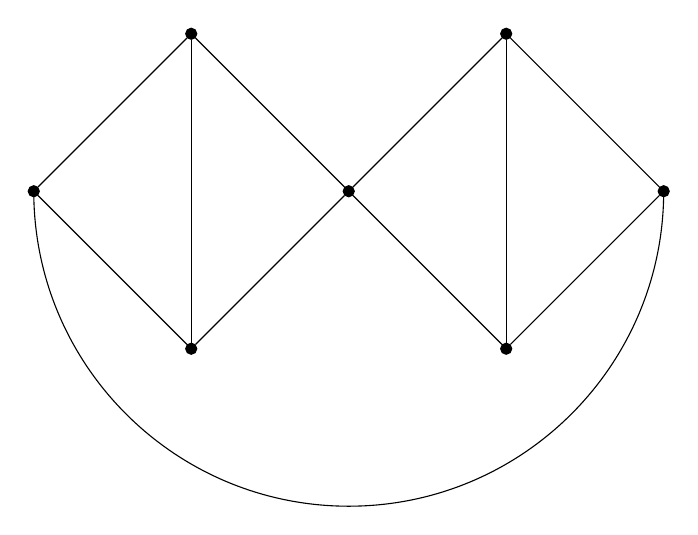
\begin{tikzpicture}
\begin{scope}
		[vertex/.style={draw,circle,inner sep = 0em, minimum size = 0.4em, fill=black},
		 edgelabel/.style = {fill = white, inner sep = 0.1em, font=\small}]
		\node[vertex] (a) at (0,0) {};
		\node[vertex] (b) at (4,0) {};
		\node[vertex] (c) at (-2,-2) {};
		\node[vertex] (d) at (2,-2) {};
		\node[vertex] (e) at (6,-2) {};
		\node[vertex] (f) at (0,-4) {};
		\node[vertex] (g) at (4,-4) {};
		
		\draw[-] (a) to (c);
		\draw[-] (a) to (d);
		\draw[-] (b) to (d);
		\draw[-] (b) to (e);
		\draw[-] (f) to (c);
		\draw[-] (f) to (d);
		\draw[-] (g) to (d);
		\draw[-] (g) to (e);
		\draw[-] (b) to (g);
		\draw[-] (a) to (f);
		\draw (-2, -2) arc (-180:0:4);
		
\end{scope}
\end{tikzpicture}
\end{document}